% Options for packages loaded elsewhere
\PassOptionsToPackage{unicode}{hyperref}
\PassOptionsToPackage{hyphens}{url}
\PassOptionsToPackage{dvipsnames,svgnames*,x11names*}{xcolor}
%
\documentclass[
  ignorenonframetext,
]{beamer}
\usepackage{pgfpages}
\setbeamertemplate{caption}[numbered]
\setbeamertemplate{caption label separator}{: }
\setbeamercolor{caption name}{fg=normal text.fg}
\beamertemplatenavigationsymbolsempty
% Prevent slide breaks in the middle of a paragraph
\widowpenalties 1 10000
\raggedbottom
\setbeamertemplate{part page}{
  \centering
  \begin{beamercolorbox}[sep=16pt,center]{part title}
    \usebeamerfont{part title}\insertpart\par
  \end{beamercolorbox}
}
\setbeamertemplate{section page}{
  \centering
  \begin{beamercolorbox}[sep=12pt,center]{part title}
    \usebeamerfont{section title}\insertsection\par
  \end{beamercolorbox}
}
\setbeamertemplate{subsection page}{
  \centering
  \begin{beamercolorbox}[sep=8pt,center]{part title}
    \usebeamerfont{subsection title}\insertsubsection\par
  \end{beamercolorbox}
}
\AtBeginPart{
  \frame{\partpage}
}
\AtBeginSection{
  \ifbibliography
  \else
    \frame{\sectionpage}
  \fi
}
\AtBeginSubsection{
  \frame{\subsectionpage}
}
\usepackage{lmodern}
\usepackage{amssymb,amsmath}
\usepackage{ifxetex,ifluatex}
\ifnum 0\ifxetex 1\fi\ifluatex 1\fi=0 % if pdftex
  \usepackage[T1]{fontenc}
  \usepackage[utf8]{inputenc}
  \usepackage{textcomp} % provide euro and other symbols
\else % if luatex or xetex
  \usepackage{unicode-math}
  \defaultfontfeatures{Scale=MatchLowercase}
  \defaultfontfeatures[\rmfamily]{Ligatures=TeX,Scale=1}
\fi
% Use upquote if available, for straight quotes in verbatim environments
\IfFileExists{upquote.sty}{\usepackage{upquote}}{}
\IfFileExists{microtype.sty}{% use microtype if available
  \usepackage[]{microtype}
  \UseMicrotypeSet[protrusion]{basicmath} % disable protrusion for tt fonts
}{}
\makeatletter
\@ifundefined{KOMAClassName}{% if non-KOMA class
  \IfFileExists{parskip.sty}{%
    \usepackage{parskip}
  }{% else
    \setlength{\parindent}{0pt}
    \setlength{\parskip}{6pt plus 2pt minus 1pt}}
}{% if KOMA class
  \KOMAoptions{parskip=half}}
\makeatother
\usepackage{xcolor}
\IfFileExists{xurl.sty}{\usepackage{xurl}}{} % add URL line breaks if available
\IfFileExists{bookmark.sty}{\usepackage{bookmark}}{\usepackage{hyperref}}
\hypersetup{
  pdftitle={Likelihood and Model Evaluation},
  pdfauthor={Zack Treisman},
  colorlinks=true,
  linkcolor=Maroon,
  filecolor=Maroon,
  citecolor=blue,
  urlcolor=Blue,
  pdfcreator={LaTeX via pandoc}}
\urlstyle{same} % disable monospaced font for URLs
\newif\ifbibliography
\usepackage{color}
\usepackage{fancyvrb}
\newcommand{\VerbBar}{|}
\newcommand{\VERB}{\Verb[commandchars=\\\{\}]}
\DefineVerbatimEnvironment{Highlighting}{Verbatim}{commandchars=\\\{\}}
% Add ',fontsize=\small' for more characters per line
\usepackage{framed}
\definecolor{shadecolor}{RGB}{248,248,248}
\newenvironment{Shaded}{\begin{snugshade}}{\end{snugshade}}
\newcommand{\AlertTok}[1]{\textcolor[rgb]{0.94,0.16,0.16}{#1}}
\newcommand{\AnnotationTok}[1]{\textcolor[rgb]{0.56,0.35,0.01}{\textbf{\textit{#1}}}}
\newcommand{\AttributeTok}[1]{\textcolor[rgb]{0.77,0.63,0.00}{#1}}
\newcommand{\BaseNTok}[1]{\textcolor[rgb]{0.00,0.00,0.81}{#1}}
\newcommand{\BuiltInTok}[1]{#1}
\newcommand{\CharTok}[1]{\textcolor[rgb]{0.31,0.60,0.02}{#1}}
\newcommand{\CommentTok}[1]{\textcolor[rgb]{0.56,0.35,0.01}{\textit{#1}}}
\newcommand{\CommentVarTok}[1]{\textcolor[rgb]{0.56,0.35,0.01}{\textbf{\textit{#1}}}}
\newcommand{\ConstantTok}[1]{\textcolor[rgb]{0.00,0.00,0.00}{#1}}
\newcommand{\ControlFlowTok}[1]{\textcolor[rgb]{0.13,0.29,0.53}{\textbf{#1}}}
\newcommand{\DataTypeTok}[1]{\textcolor[rgb]{0.13,0.29,0.53}{#1}}
\newcommand{\DecValTok}[1]{\textcolor[rgb]{0.00,0.00,0.81}{#1}}
\newcommand{\DocumentationTok}[1]{\textcolor[rgb]{0.56,0.35,0.01}{\textbf{\textit{#1}}}}
\newcommand{\ErrorTok}[1]{\textcolor[rgb]{0.64,0.00,0.00}{\textbf{#1}}}
\newcommand{\ExtensionTok}[1]{#1}
\newcommand{\FloatTok}[1]{\textcolor[rgb]{0.00,0.00,0.81}{#1}}
\newcommand{\FunctionTok}[1]{\textcolor[rgb]{0.00,0.00,0.00}{#1}}
\newcommand{\ImportTok}[1]{#1}
\newcommand{\InformationTok}[1]{\textcolor[rgb]{0.56,0.35,0.01}{\textbf{\textit{#1}}}}
\newcommand{\KeywordTok}[1]{\textcolor[rgb]{0.13,0.29,0.53}{\textbf{#1}}}
\newcommand{\NormalTok}[1]{#1}
\newcommand{\OperatorTok}[1]{\textcolor[rgb]{0.81,0.36,0.00}{\textbf{#1}}}
\newcommand{\OtherTok}[1]{\textcolor[rgb]{0.56,0.35,0.01}{#1}}
\newcommand{\PreprocessorTok}[1]{\textcolor[rgb]{0.56,0.35,0.01}{\textit{#1}}}
\newcommand{\RegionMarkerTok}[1]{#1}
\newcommand{\SpecialCharTok}[1]{\textcolor[rgb]{0.00,0.00,0.00}{#1}}
\newcommand{\SpecialStringTok}[1]{\textcolor[rgb]{0.31,0.60,0.02}{#1}}
\newcommand{\StringTok}[1]{\textcolor[rgb]{0.31,0.60,0.02}{#1}}
\newcommand{\VariableTok}[1]{\textcolor[rgb]{0.00,0.00,0.00}{#1}}
\newcommand{\VerbatimStringTok}[1]{\textcolor[rgb]{0.31,0.60,0.02}{#1}}
\newcommand{\WarningTok}[1]{\textcolor[rgb]{0.56,0.35,0.01}{\textbf{\textit{#1}}}}
\usepackage{graphicx,grffile}
\makeatletter
\def\maxwidth{\ifdim\Gin@nat@width>\linewidth\linewidth\else\Gin@nat@width\fi}
\def\maxheight{\ifdim\Gin@nat@height>\textheight\textheight\else\Gin@nat@height\fi}
\makeatother
% Scale images if necessary, so that they will not overflow the page
% margins by default, and it is still possible to overwrite the defaults
% using explicit options in \includegraphics[width, height, ...]{}
\setkeys{Gin}{width=\maxwidth,height=\maxheight,keepaspectratio}
% Set default figure placement to htbp
\makeatletter
\def\fps@figure{htbp}
\makeatother
\setlength{\emergencystretch}{3em} % prevent overfull lines
\providecommand{\tightlist}{%
  \setlength{\itemsep}{0pt}\setlength{\parskip}{0pt}}
\setcounter{secnumdepth}{-\maxdimen} % remove section numbering

\pgfdeclareimage[width=3.5cm]{mcslogo}{../western_logo_hor_MCS_3C_pos.pdf}
\pgfdeclareimage[width=1cm]{ccbysa}{../ccbysa88x31.png}
\titlegraphic{\href{http://creativecommons.org/licenses/by-sa/4.0/}{\pgfuseimage{ccbysa}}
\hfill
\href{https://western.edu/program/mathematics/}{\pgfuseimage{mcslogo}}}
%\usecolortheme{wcu}
%\institute{Western Colorado University}
%\setbeamertemplate{navigation symbols}{}

\title{Likelihood and Model Evaluation}
\author{Zack Treisman}
\date{Spring 2021}

\begin{document}
\frame{\titlepage}

\begin{frame}{Philosophy}
\protect\hypertarget{philosophy}{}

The time has come for us to discuss in some detail how our models are
being constructed and evaluated.

\begin{itemize}
\tightlist
\item
  The key idea is \textbf{likelihood}, the probability that a model
  would produce the data we observe.
\end{itemize}

When do we say \emph{likelihood} instead of \emph{probability}?

\begin{itemize}
\tightlist
\item
  The probability \(P(\text{data}|\text{model})\) considers the model as
  fixed, and the data as variable.
\item
  The likelihood \(\mathcal{L}(\text{model}|\text{data})\) considers the
  data to be fixed (they are what has been observed) and the model as
  variable.
\end{itemize}

This kind of model-space/ data-space parameter duality is all over the
place in math, so it must be kind of important. But this is not a class
for that sort of \emph{abstract
nonsense}\footnote{A technical term. No seriously.}.

\end{frame}

\begin{frame}{Maximum Likelihood Estimation}
\protect\hypertarget{maximum-likelihood-estimation}{}

To find a parametric model to fit data we need to choose values for the
parameters according to some criteria.

\begin{itemize}
\tightlist
\item
  Minimizing mean squared error is ideal if the true error distribution
  is normal with constant variance.
\item
  Non-normal errors are modeled with a GLM.
\item
  Heterogenous variance can be accounted for by a mixed/ multilevel
  model. (Coming soon)
\item
  Finding parameters by maximizing the likelihood agrees with least
  squares when errors are normal and homoscedastic gives good results
  when they are not.
\end{itemize}

\end{frame}

\begin{frame}[fragile]{Computing likelihood}
\protect\hypertarget{computing-likelihood}{}

Since likelihoods are just probabilities with a shift in what we
consider to be a variable, we have the tools to compute them.

\scriptsize

\begin{Shaded}
\begin{Highlighting}[]
\NormalTok{x <-}\StringTok{ }\KeywordTok{subset}\NormalTok{(ReedfrogPred,pred}\OperatorTok{==}\StringTok{"pred"} \OperatorTok{&}\StringTok{ }\NormalTok{density}\OperatorTok{==}\DecValTok{10} \OperatorTok{&}\StringTok{ }\NormalTok{size}\OperatorTok{==}\StringTok{"small"}\NormalTok{)}
\NormalTok{x}
\end{Highlighting}
\end{Shaded}

\begin{verbatim}
##    density pred  size surv propsurv
## 13      10 pred small    7      0.7
## 14      10 pred small    5      0.5
## 15      10 pred small    9      0.9
## 16      10 pred small    9      0.9
\end{verbatim}

\begin{Shaded}
\begin{Highlighting}[]
\NormalTok{likhd_indiv <-}\StringTok{ }\KeywordTok{dbinom}\NormalTok{(x}\OperatorTok{$}\NormalTok{surv, x}\OperatorTok{$}\NormalTok{density, }\DataTypeTok{p=}\FloatTok{0.7}\NormalTok{)}
\NormalTok{likhd_indiv}
\end{Highlighting}
\end{Shaded}

\begin{verbatim}
## [1] 0.2668279 0.1029193 0.1210608 0.1210608
\end{verbatim}

\begin{Shaded}
\begin{Highlighting}[]
\NormalTok{likhd <-}\StringTok{ }\KeywordTok{prod}\NormalTok{(likhd_indiv)}
\NormalTok{likhd}
\end{Highlighting}
\end{Shaded}

\begin{verbatim}
## [1] 0.0004024719
\end{verbatim}

\end{frame}

\begin{frame}[fragile]{Optimizing}
\protect\hypertarget{optimizing}{}

Given a parameter and a function of that parameter, the \texttt{optim}
command searches for the value of the parameter that gives the optimal
(minimum or maximum) value of the function. \scriptsize

\begin{Shaded}
\begin{Highlighting}[]
\NormalTok{likhd_fn <-}\StringTok{ }\ControlFlowTok{function}\NormalTok{(p)\{}\KeywordTok{prod}\NormalTok{(}\KeywordTok{dbinom}\NormalTok{(x}\OperatorTok{$}\NormalTok{surv, x}\OperatorTok{$}\NormalTok{density, }\DataTypeTok{p=}\NormalTok{p))\}}
\NormalTok{opt0 <-}\StringTok{ }\KeywordTok{optim}\NormalTok{(}\DataTypeTok{fn =}\NormalTok{ likhd_fn, }\DataTypeTok{par =} \KeywordTok{list}\NormalTok{(}\DataTypeTok{p=}\FloatTok{0.7}\NormalTok{), }
              \DataTypeTok{control=}\KeywordTok{list}\NormalTok{(}\DataTypeTok{fnscale=}\OperatorTok{-}\DecValTok{1}\NormalTok{), }\CommentTok{#maximize instead of minimize}
              \DataTypeTok{method=}\StringTok{"BFGS"}\NormalTok{) }\CommentTok{#better for one variable}
\NormalTok{opt0}\OperatorTok{$}\NormalTok{par}
\end{Highlighting}
\end{Shaded}

\begin{verbatim}
##         p 
## 0.7499974
\end{verbatim}

\begin{Shaded}
\begin{Highlighting}[]
\KeywordTok{sum}\NormalTok{(x}\OperatorTok{$}\NormalTok{surv)}\OperatorTok{/}\KeywordTok{sum}\NormalTok{(x}\OperatorTok{$}\NormalTok{density)}
\end{Highlighting}
\end{Shaded}

\begin{verbatim}
## [1] 0.75
\end{verbatim}

\end{frame}

\begin{frame}[fragile]{Negative log-likelihoods}
\protect\hypertarget{negative-log-likelihoods}{}

For computational reasons, it is easier to deal with the logs of
likelihood values.

\begin{itemize}
\tightlist
\item
  Products of more than a few numbers between 0 and 1 get really small.
\item
  Logs turn products into sums.
\end{itemize}

For emotional reasons, it's easier to minimize than to maximize.

\begin{itemize}
\tightlist
\item
  Because gravity?
\end{itemize}

Replace \texttt{prod} with \texttt{-sum} and add in \texttt{log=TRUE}.
Same result.

\scriptsize

\begin{Shaded}
\begin{Highlighting}[]
\NormalTok{nll_fn <-}\StringTok{ }\ControlFlowTok{function}\NormalTok{(p)\{}\OperatorTok{-}\KeywordTok{sum}\NormalTok{(}\KeywordTok{dbinom}\NormalTok{(x}\OperatorTok{$}\NormalTok{surv, x}\OperatorTok{$}\NormalTok{density, }\DataTypeTok{p=}\NormalTok{p, }\DataTypeTok{log =} \OtherTok{TRUE}\NormalTok{))\}}
\NormalTok{opt1 <-}\StringTok{ }\KeywordTok{optim}\NormalTok{(}\DataTypeTok{fn =}\NormalTok{ nll_fn, }\DataTypeTok{par =} \KeywordTok{list}\NormalTok{(}\DataTypeTok{p=}\FloatTok{0.7}\NormalTok{), }
              \DataTypeTok{method=}\StringTok{"BFGS"}\NormalTok{) }\CommentTok{#better for one variable}
\NormalTok{opt1}\OperatorTok{$}\NormalTok{par}
\end{Highlighting}
\end{Shaded}

\begin{verbatim}
##         p 
## 0.7500001
\end{verbatim}

\end{frame}

\begin{frame}[fragile]{The \texttt{mle2} command}
\protect\hypertarget{the-mle2-command}{}

The \texttt{bbmle} package provides \texttt{mle2} for maximum likelihood
estimates.

\scriptsize

\begin{Shaded}
\begin{Highlighting}[]
\CommentTok{#library(bbmle)}
\KeywordTok{mle2}\NormalTok{(nll_fn, }\DataTypeTok{start =} \KeywordTok{list}\NormalTok{(}\DataTypeTok{p=}\FloatTok{0.7}\NormalTok{), }\DataTypeTok{data=}\NormalTok{x)}
\end{Highlighting}
\end{Shaded}

\begin{verbatim}
## 
## Call:
## mle2(minuslogl = nll_fn, start = list(p = 0.7), data = x)
## 
## Coefficients:
##         p 
## 0.7500001 
## 
## Log-likelihood: -7.57
\end{verbatim}

\end{frame}

\begin{frame}[fragile]{MLE agrees with ordinary least squares}
\protect\hypertarget{mle-agrees-with-ordinary-least-squares}{}

\scriptsize

\begin{Shaded}
\begin{Highlighting}[]
\NormalTok{x<-}\KeywordTok{rnorm}\NormalTok{(}\DecValTok{50}\NormalTok{,}\DecValTok{5}\NormalTok{,}\DecValTok{1}\NormalTok{)}
\NormalTok{y<-}\KeywordTok{rnorm}\NormalTok{(}\DecValTok{50}\NormalTok{, }\DecValTok{3}\OperatorTok{+}\DecValTok{2}\OperatorTok{*}\NormalTok{x,}\FloatTok{1.5}\NormalTok{)}
\KeywordTok{lm}\NormalTok{(y}\OperatorTok{~}\NormalTok{x)}
\end{Highlighting}
\end{Shaded}

\begin{verbatim}
## 
## Call:
## lm(formula = y ~ x)
## 
## Coefficients:
## (Intercept)            x  
##       2.369        2.124
\end{verbatim}

\begin{Shaded}
\begin{Highlighting}[]
\NormalTok{nll_fn <-}\StringTok{ }\ControlFlowTok{function}\NormalTok{(a,b,s) }\OperatorTok{-}\KeywordTok{sum}\NormalTok{(}\KeywordTok{dnorm}\NormalTok{(y, a}\OperatorTok{+}\NormalTok{b}\OperatorTok{*}\NormalTok{x, s, }\DataTypeTok{log =} \OtherTok{TRUE}\NormalTok{))}
\KeywordTok{mle2}\NormalTok{(nll_fn, }\DataTypeTok{start =} \KeywordTok{list}\NormalTok{(}\DataTypeTok{a=}\DecValTok{2}\NormalTok{,}\DataTypeTok{b=}\DecValTok{3}\NormalTok{,}\DataTypeTok{s=}\DecValTok{1}\NormalTok{))}
\end{Highlighting}
\end{Shaded}

\begin{verbatim}
## 
## Call:
## mle2(minuslogl = nll_fn, start = list(a = 2, b = 3, s = 1))
## 
## Coefficients:
##        a        b        s 
## 2.369030 2.124338 1.520781 
## 
## Log-likelihood: -91.91
\end{verbatim}

\end{frame}

\begin{frame}[fragile]{MLE is used to fit a GLM}
\protect\hypertarget{mle-is-used-to-fit-a-glm}{}

\scriptsize

\begin{Shaded}
\begin{Highlighting}[]
\NormalTok{n <-}\StringTok{ }\DecValTok{50}\NormalTok{; x <-}\StringTok{ }\KeywordTok{runif}\NormalTok{(n, }\DataTypeTok{min=}\DecValTok{0}\NormalTok{, }\DataTypeTok{max=}\DecValTok{5}\NormalTok{); y <-}\StringTok{ }\KeywordTok{rpois}\NormalTok{(n, }\DecValTok{2}\OperatorTok{+}\NormalTok{x)}
\NormalTok{glm1 <-}\StringTok{ }\KeywordTok{glm}\NormalTok{(y}\OperatorTok{~}\NormalTok{x, }\DataTypeTok{family =}\NormalTok{ poisson)}
\KeywordTok{coef}\NormalTok{(glm1)}
\end{Highlighting}
\end{Shaded}

\begin{verbatim}
## (Intercept)           x 
##   1.1163184   0.1657753
\end{verbatim}

\normalsize

\begin{itemize}
\tightlist
\item
  In \texttt{mle2} both the negative log-likelihood function and the
  parameters can be expressed as formulae.
\end{itemize}

\scriptsize

\begin{Shaded}
\begin{Highlighting}[]
\KeywordTok{mle2}\NormalTok{(y}\OperatorTok{~}\KeywordTok{dpois}\NormalTok{(}\KeywordTok{exp}\NormalTok{(loglambda)),       }\CommentTok{## use log link/exp inverse-link}
     \DataTypeTok{data=}\KeywordTok{data.frame}\NormalTok{(y,x),          }\CommentTok{## need to specify as data frame}
     \DataTypeTok{parameters=}\KeywordTok{list}\NormalTok{(loglambda}\OperatorTok{~}\NormalTok{x),  }\CommentTok{## linear model for loglambda}
     \DataTypeTok{start=}\KeywordTok{list}\NormalTok{(}\DataTypeTok{loglambda=}\DecValTok{0}\NormalTok{))       }\CommentTok{## start values for *intercept*}
\end{Highlighting}
\end{Shaded}

\begin{verbatim}
## 
## Call:
## mle2(minuslogl = y ~ dpois(exp(loglambda)), start = list(loglambda = 0), 
##     data = data.frame(y, x), parameters = list(loglambda ~ x))
## 
## Coefficients:
## loglambda.(Intercept)           loglambda.x 
##             1.1163260             0.1657724 
## 
## Log-likelihood: -104.72
\end{verbatim}

\end{frame}

\begin{frame}[fragile]{A plot of \texttt{glm1}}
\protect\hypertarget{a-plot-of-glm1}{}

Always plot your data and models. \scriptsize

\begin{Shaded}
\begin{Highlighting}[]
\KeywordTok{ggplot}\NormalTok{(}\KeywordTok{data.frame}\NormalTok{(}\DataTypeTok{x=}\NormalTok{x, }\DataTypeTok{y=}\NormalTok{y), }\KeywordTok{aes}\NormalTok{(x,y))}\OperatorTok{+}
\StringTok{  }\KeywordTok{geom_point}\NormalTok{()}\OperatorTok{+}
\StringTok{  }\KeywordTok{geom_line}\NormalTok{(}\KeywordTok{aes}\NormalTok{(}\DataTypeTok{y=}\KeywordTok{exp}\NormalTok{(}\KeywordTok{predict}\NormalTok{(glm1))))}\OperatorTok{+}
\StringTok{  }\KeywordTok{geom_line}\NormalTok{(}\KeywordTok{aes}\NormalTok{(}\DataTypeTok{y=}\KeywordTok{qpois}\NormalTok{(}\FloatTok{0.025}\NormalTok{,}\DataTypeTok{lambda =} \KeywordTok{exp}\NormalTok{(}\KeywordTok{predict}\NormalTok{(glm1)))), }\DataTypeTok{linetype=}\DecValTok{2}\NormalTok{)}\OperatorTok{+}
\StringTok{  }\KeywordTok{geom_line}\NormalTok{(}\KeywordTok{aes}\NormalTok{(}\DataTypeTok{y=}\KeywordTok{qpois}\NormalTok{(}\FloatTok{0.975}\NormalTok{,}\DataTypeTok{lambda =} \KeywordTok{exp}\NormalTok{(}\KeywordTok{predict}\NormalTok{(glm1)))), }\DataTypeTok{linetype=}\DecValTok{2}\NormalTok{)}
\end{Highlighting}
\end{Shaded}

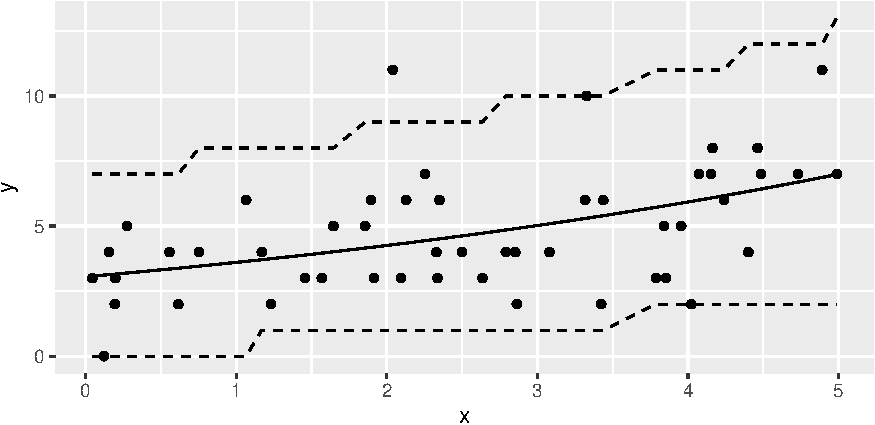
\includegraphics{likelihood_files/figure-beamer/unnamed-chunk-9-1.pdf}

\end{frame}

\begin{frame}[fragile]{Analysis of a GLM}
\protect\hypertarget{analysis-of-a-glm}{}

\scriptsize

\begin{Shaded}
\begin{Highlighting}[]
\KeywordTok{summary}\NormalTok{(glm1)}
\end{Highlighting}
\end{Shaded}

\begin{verbatim}
## 
## Call:
## glm(formula = y ~ x, family = poisson)
## 
## Deviance Residuals: 
##      Min        1Q    Median        3Q       Max  
## -2.49652  -0.65872  -0.05523   0.45253   2.70580  
## 
## Coefficients:
##             Estimate Std. Error z value Pr(>|z|)    
## (Intercept)  1.11632    0.14679   7.605 2.85e-14 ***
## x            0.16578    0.04588   3.614 0.000302 ***
## ---
## Signif. codes:  0 '***' 0.001 '**' 0.01 '*' 0.05 '.' 0.1 ' ' 1
## 
## (Dispersion parameter for poisson family taken to be 1)
## 
##     Null deviance: 58.191  on 49  degrees of freedom
## Residual deviance: 44.789  on 48  degrees of freedom
## AIC: 213.43
## 
## Number of Fisher Scoring iterations: 4
\end{verbatim}

\end{frame}

\begin{frame}{Deviance}
\protect\hypertarget{deviance}{}

In general, the deviance compares any two models. Here, the fitted glm
is compared to a model perfectly overfit to the sample.

\begin{itemize}
\tightlist
\item
  This perfect model is known as the saturated model, or the Bayes
  optimal model.
\item
  The responses \(f_{sat}(x_i)\) equal the observed responses \(y_i\),
  or \(f_{sat}(x_i)\) is the mean of the relevant \(y_i\) if there are
  multiple observations with the same \(x_i\).
\end{itemize}

In code: \[
f_{sat}(x_i)=\tt{mean(y[x==xi])}
\]

Deviance is the difference between the log-likelihoods of the fitted and
saturated models. Times -2. \[
D=-2(L(\text{model})-L_{sat})
\] Deviance acts kind of like variance. Since likelihood is computed as
a sum of contributions from each data point, it's easy to split total
deviance into \emph{residual deviances}.

\end{frame}

\begin{frame}{Dispersion}
\protect\hypertarget{dispersion}{}

For the models of the lily data we computed the ratio of residual
deviance to degrees of freedom and compared this ratio to one. If this
ratio was greater than one we called the model \emph{overdispersed}.

In the Poisson distribution, the mean equals the variance, which ends up
being really restrictive.

\end{frame}

\begin{frame}[fragile]{Null and residual deviance and how they connect
to degrees of freedom}
\protect\hypertarget{null-and-residual-deviance-and-how-they-connect-to-degrees-of-freedom}{}

The null deviance is the deviance of the null model

\texttt{glm(y\textasciitilde{}1,\ family=poisson)}

and the residual deviance is the deviance of the fitted model

\texttt{glm(y\textasciitilde{}x,\ family=poisson)}.

Dividing by degrees of freedom puts these on the same scale in a
``number of ways to alter the model'' sense of same.

\end{frame}

\begin{frame}[fragile]{Likelihood and AIC}
\protect\hypertarget{likelihood-and-aic}{}

Akaike's Information Criterion is the negative log-likelihood plus a
penalty term for each coefficient that is estimated in the model. Times
2.

\begin{Shaded}
\begin{Highlighting}[]
\NormalTok{L <-}\StringTok{ }\KeywordTok{logLik}\NormalTok{(glm1)[}\DecValTok{1}\NormalTok{]}
\NormalTok{L}
\end{Highlighting}
\end{Shaded}

\begin{verbatim}
## [1] -104.7164
\end{verbatim}

\begin{Shaded}
\begin{Highlighting}[]
\NormalTok{k <-}\StringTok{ }\KeywordTok{length}\NormalTok{(}\KeywordTok{coef}\NormalTok{(glm1))}
\NormalTok{k}
\end{Highlighting}
\end{Shaded}

\begin{verbatim}
## [1] 2
\end{verbatim}

\begin{Shaded}
\begin{Highlighting}[]
\DecValTok{-2}\OperatorTok{*}\NormalTok{L}\OperatorTok{+}\DecValTok{2}\OperatorTok{*}\NormalTok{k}
\end{Highlighting}
\end{Shaded}

\begin{verbatim}
## [1] 213.4329
\end{verbatim}

\begin{Shaded}
\begin{Highlighting}[]
\KeywordTok{AIC}\NormalTok{(glm1)}
\end{Highlighting}
\end{Shaded}

\begin{verbatim}
## [1] 213.4329
\end{verbatim}

\end{frame}

\begin{frame}{Interpreting AIC}
\protect\hypertarget{interpreting-aic}{}

Given a set of \(M\) different models
\(\text{mod}_1,\ldots,\text{mod}_M\) write \(AIC_i\) for the AIC of the
\(i^{th}\) model and \(AIC_{min}\) for the smallest of these values.

\begin{itemize}
\item
  Define \(\Delta_i=AIC_i-AIC_{min}\). These differences in AIC values
  are more relevant than the actual AICs.
\item
  An estimate of the relative likelihood of model \(i\) is
  \(\exp\left(-\frac{\Delta_i}{2}\right)\). These are sometimes called
  \emph{evidence ratios}.
\item
  Scaling the relative likelihoods by the sum of the relative
  likelihoods for all models in consideration give the AIC weight. \[
  w_i=\frac{\exp\left(-\frac{\Delta_i}{2}\right)}{\sum_{j=i}^{M}\exp\left(-\frac{\Delta_j}{2}\right)}
  \]
\end{itemize}

This is roughly interpretable as the probability that the \(i^{th}\)
model is the best model.

\end{frame}

\begin{frame}{Customary meanings for differences in AIC}
\protect\hypertarget{customary-meanings-for-differences-in-aic}{}

There are no definite meanings for differences in AIC, but the following
are somewhat customary interpretations.

\begin{itemize}
\tightlist
\item
  Models with \(\Delta<2\) are basically indistinguishable from the
  model with \(AIC_{min}\).
\item
  Models with \(\Delta>10\) are much less predictive or explanatory than
  the model with \(AIC_{min}\).
\item
  For \(2<\Delta<10\) there are a variety of adjectives used to describe
  model quality.
\end{itemize}

\end{frame}

\begin{frame}[fragile]{Other information critera}
\protect\hypertarget{other-information-critera}{}

Other options exist, they are also all modifications of the likelihood,
and behave and are interpreted similarly to AIC.

\begin{Shaded}
\begin{Highlighting}[]
\KeywordTok{AIC}\NormalTok{(glm1)}\OperatorTok{+}\DecValTok{2}\OperatorTok{*}\NormalTok{k}\OperatorTok{*}\NormalTok{(k}\OperatorTok{+}\DecValTok{1}\NormalTok{)}\OperatorTok{/}\NormalTok{(n}\OperatorTok{-}\NormalTok{k}\DecValTok{-1}\NormalTok{)}
\end{Highlighting}
\end{Shaded}

\begin{verbatim}
## [1] 213.6882
\end{verbatim}

\begin{Shaded}
\begin{Highlighting}[]
\KeywordTok{AICc}\NormalTok{(glm1) }\CommentTok{#from MuMIn. bbmle's doesn't work on glm}
\end{Highlighting}
\end{Shaded}

\begin{verbatim}
## [1] 213.6882
\end{verbatim}

\begin{Shaded}
\begin{Highlighting}[]
\DecValTok{-2}\OperatorTok{*}\NormalTok{L}\OperatorTok{+}\KeywordTok{log}\NormalTok{(n)}\OperatorTok{*}\NormalTok{k}
\end{Highlighting}
\end{Shaded}

\begin{verbatim}
## [1] 217.2569
\end{verbatim}

\begin{Shaded}
\begin{Highlighting}[]
\KeywordTok{BIC}\NormalTok{(glm1)}
\end{Highlighting}
\end{Shaded}

\begin{verbatim}
## [1] 217.2569
\end{verbatim}

\end{frame}

\begin{frame}{Fisher scoring iterations}
\protect\hypertarget{fisher-scoring-iterations}{}

Fisher's method of iteratively adjusting the parameters to get an
increase in maximum likelihood is how the job is done. The number of
iterations is how long it took to converge.

\end{frame}

\begin{frame}[fragile]{Other applications of likelihood}
\protect\hypertarget{other-applications-of-likelihood}{}

\begin{itemize}
\tightlist
\item
  Likelihood ratio tests
\end{itemize}

These can be implemented using the \texttt{anova} command on a
\texttt{glm} and specifying \texttt{test="LRT"}. See
\texttt{?anova.glm}. There is also the command \texttt{drop1} if you
want to do the equivalent of marginal instead of sequential ANOVA.

\begin{itemize}
\tightlist
\item
  Bayesian analysis
\end{itemize}

The likelihood is a key element in Bayesian analysis, which takes the
idea that model parameters are the real variables, and the data are the
values that we really know and runs with it.

\end{frame}

\begin{frame}[fragile]{Likelihood ratio tests}
\protect\hypertarget{likelihood-ratio-tests}{}

\scriptsize

\begin{Shaded}
\begin{Highlighting}[]
\NormalTok{x1 <-}\StringTok{ }\KeywordTok{runif}\NormalTok{(n, }\DataTypeTok{min=}\DecValTok{0}\NormalTok{, }\DataTypeTok{max=}\DecValTok{5}\NormalTok{); x2 <-}\StringTok{ }\KeywordTok{runif}\NormalTok{(n, }\DataTypeTok{min=}\DecValTok{0}\NormalTok{, }\DataTypeTok{max=}\DecValTok{10}\NormalTok{)}
\NormalTok{y <-}\StringTok{ }\KeywordTok{rpois}\NormalTok{(n, }\DecValTok{2}\OperatorTok{+}\DecValTok{2}\OperatorTok{*}\NormalTok{x1}\OperatorTok{+}\NormalTok{x2)}
\NormalTok{glm2interact <-}\StringTok{ }\KeywordTok{glm}\NormalTok{(y}\OperatorTok{~}\NormalTok{x1}\OperatorTok{*}\NormalTok{x2, }\DataTypeTok{family =}\NormalTok{ poisson)}
\NormalTok{glm2both <-}\StringTok{ }\KeywordTok{glm}\NormalTok{(y}\OperatorTok{~}\NormalTok{x1}\OperatorTok{+}\NormalTok{x2, }\DataTypeTok{family =}\NormalTok{ poisson)}
\NormalTok{glm2x1 <-}\StringTok{ }\KeywordTok{glm}\NormalTok{(y}\OperatorTok{~}\NormalTok{x1, }\DataTypeTok{family =}\NormalTok{ poisson)}
\NormalTok{glm2x2 <-}\StringTok{ }\KeywordTok{glm}\NormalTok{(y}\OperatorTok{~}\NormalTok{x2, }\DataTypeTok{family=}\NormalTok{poisson)}
\NormalTok{glm2null <-}\StringTok{ }\KeywordTok{glm}\NormalTok{(y}\OperatorTok{~}\DecValTok{1}\NormalTok{, }\DataTypeTok{family =}\NormalTok{ poisson)}
\KeywordTok{anova}\NormalTok{(glm2null,glm2x1,glm2both, glm2interact, }\DataTypeTok{test=}\StringTok{"LRT"}\NormalTok{)}
\end{Highlighting}
\end{Shaded}

\begin{verbatim}
## Analysis of Deviance Table
## 
## Model 1: y ~ 1
## Model 2: y ~ x1
## Model 3: y ~ x1 + x2
## Model 4: y ~ x1 * x2
##   Resid. Df Resid. Dev Df Deviance  Pr(>Chi)    
## 1        49    109.501                          
## 2        48     78.220  1   31.281 2.233e-08 ***
## 3        47     39.739  1   38.482 5.527e-10 ***
## 4        46     36.655  1    3.084   0.07907 .  
## ---
## Signif. codes:  0 '***' 0.001 '**' 0.01 '*' 0.05 '.' 0.1 ' ' 1
\end{verbatim}

\end{frame}

\begin{frame}[fragile]{Other applications of \texttt{mle2}}
\protect\hypertarget{other-applications-of-mle2}{}

This tool can do maximum likelihood estimation to find parameters for
many sorts of models that \texttt{glm} can't. It's tricky to use, and
can rely in unexpected ways on the \texttt{start} values, so often it's
easier to find a prepackaged tool like \texttt{glm}.

But if you know exactly the model you want to build and have good
guesses for the parameters that you hope to estimate, this could be the
tool for you.

\end{frame}

\begin{frame}{Things in \texttt{summary.lm} but not
\texttt{summary.glm}}
\protect\hypertarget{things-in-summary.lm-but-not-summary.glm}{}

There are two things that we are missing.

\begin{itemize}
\tightlist
\item
  \(R^2\)
\end{itemize}

There's no consensus about what we can or should use to replace \(R^2\).
There's a good discussion of this by Bolker here:
{[}\url{https://bbolker.github.io/mixedmodels-misc/glmmFAQ.html\#how-do-i-compute-a-coefficient-of-determination-r2-or-an-analogue-for-glmms}{]}

\begin{itemize}
\tightlist
\item
  An overall p-value.
\end{itemize}

There's no obvious replacement for \(F\), or clear reason why we can't
keep using \(F\). But since there are likelihood ratios (and other
metrics of goodness-of-fit) it would be presumptuous to give an overall
p-value based on an \(F\) test.

\end{frame}

\end{document}
